\documentclass[twoside]{book}

% Packages required by doxygen
\usepackage{fixltx2e}
\usepackage{calc}
\usepackage{doxygen}
\usepackage[export]{adjustbox} % also loads graphicx
\usepackage{graphicx}
\usepackage[utf8]{inputenc}
\usepackage{makeidx}
\usepackage{multicol}
\usepackage{multirow}
\PassOptionsToPackage{warn}{textcomp}
\usepackage{textcomp}
\usepackage[nointegrals]{wasysym}
\usepackage[table]{xcolor}

% Font selection
\usepackage[T1]{fontenc}
\usepackage[scaled=.90]{helvet}
\usepackage{courier}
\usepackage{amssymb}
\usepackage{sectsty}
\renewcommand{\familydefault}{\sfdefault}
\allsectionsfont{%
  \fontseries{bc}\selectfont%
  \color{darkgray}%
}
\renewcommand{\DoxyLabelFont}{%
  \fontseries{bc}\selectfont%
  \color{darkgray}%
}
\newcommand{\+}{\discretionary{\mbox{\scriptsize$\hookleftarrow$}}{}{}}

% Page & text layout
\usepackage{geometry}
\geometry{%
  a4paper,%
  top=2.5cm,%
  bottom=2.5cm,%
  left=2.5cm,%
  right=2.5cm%
}
\tolerance=750
\hfuzz=15pt
\hbadness=750
\setlength{\emergencystretch}{15pt}
\setlength{\parindent}{0cm}
\setlength{\parskip}{3ex plus 2ex minus 2ex}
\makeatletter
\renewcommand{\paragraph}{%
  \@startsection{paragraph}{4}{0ex}{-1.0ex}{1.0ex}{%
    \normalfont\normalsize\bfseries\SS@parafont%
  }%
}
\renewcommand{\subparagraph}{%
  \@startsection{subparagraph}{5}{0ex}{-1.0ex}{1.0ex}{%
    \normalfont\normalsize\bfseries\SS@subparafont%
  }%
}
\makeatother

% Headers & footers
\usepackage{fancyhdr}
\pagestyle{fancyplain}
\fancyhead[LE]{\fancyplain{}{\bfseries\thepage}}
\fancyhead[CE]{\fancyplain{}{}}
\fancyhead[RE]{\fancyplain{}{\bfseries\leftmark}}
\fancyhead[LO]{\fancyplain{}{\bfseries\rightmark}}
\fancyhead[CO]{\fancyplain{}{}}
\fancyhead[RO]{\fancyplain{}{\bfseries\thepage}}
\fancyfoot[LE]{\fancyplain{}{}}
\fancyfoot[CE]{\fancyplain{}{}}
\fancyfoot[RE]{\fancyplain{}{\bfseries\scriptsize Generated by Doxygen }}
\fancyfoot[LO]{\fancyplain{}{\bfseries\scriptsize Generated by Doxygen }}
\fancyfoot[CO]{\fancyplain{}{}}
\fancyfoot[RO]{\fancyplain{}{}}
\renewcommand{\footrulewidth}{0.4pt}
\renewcommand{\chaptermark}[1]{%
  \markboth{#1}{}%
}
\renewcommand{\sectionmark}[1]{%
  \markright{\thesection\ #1}%
}

% Indices & bibliography
\usepackage{natbib}
\usepackage[titles]{tocloft}
\setcounter{tocdepth}{3}
\setcounter{secnumdepth}{5}
\makeindex

% Hyperlinks (required, but should be loaded last)
\usepackage{ifpdf}
\ifpdf
  \usepackage[pdftex,pagebackref=true]{hyperref}
\else
  \usepackage[ps2pdf,pagebackref=true]{hyperref}
\fi
\hypersetup{%
  colorlinks=true,%
  linkcolor=blue,%
  citecolor=blue,%
  unicode%
}

% Custom commands
\newcommand{\clearemptydoublepage}{%
  \newpage{\pagestyle{empty}\cleardoublepage}%
}

\usepackage{caption}
\captionsetup{labelsep=space,justification=centering,font={bf},singlelinecheck=off,skip=4pt,position=top}

%===== C O N T E N T S =====

\begin{document}

% Titlepage & ToC
\hypersetup{pageanchor=false,
             bookmarksnumbered=true,
             pdfencoding=unicode
            }
\pagenumbering{alph}
\begin{titlepage}
\vspace*{7cm}
\begin{center}%
{\Large Elevator }\\
\vspace*{1cm}
{\large Generated by Doxygen 1.8.13}\\
\end{center}
\end{titlepage}
\clearemptydoublepage
\pagenumbering{roman}
\tableofcontents
\clearemptydoublepage
\pagenumbering{arabic}
\hypersetup{pageanchor=true}

%--- Begin generated contents ---
\chapter{Data Structure Index}
\section{Data Structures}
Here are the data structures with brief descriptions\+:\begin{DoxyCompactList}
\item\contentsline{section}{\hyperlink{structelevator__t}{elevator\+\_\+t} \\*Struct that describes the elevator. It contains all the important variables for the process }{\pageref{structelevator__t}}{}
\end{DoxyCompactList}

\chapter{File Index}
\section{File List}
Here is a list of all documented files with brief descriptions\+:\begin{DoxyCompactList}
\item\contentsline{section}{source/{\bfseries elevator.\+c} }{\pageref{elevator_8c}}{}
\item\contentsline{section}{source/\hyperlink{elevator_8h}{elevator.\+h} \\*File that contains the elevator struct and basic elevator functions }{\pageref{elevator_8h}}{}
\item\contentsline{section}{source/{\bfseries elevator\+\_\+driver.\+c} }{\pageref{elevator__driver_8c}}{}
\item\contentsline{section}{source/\hyperlink{elevator__driver_8h}{elevator\+\_\+driver.\+h} \\*File that contains the functions needed for driving the elevator and getting information from the differnt sensors to upfate the floor }{\pageref{elevator__driver_8h}}{}
\item\contentsline{section}{source/{\bfseries fsm\+\_\+elevator.\+c} }{\pageref{fsm__elevator_8c}}{}
\item\contentsline{section}{source/\hyperlink{fsm__elevator_8h}{fsm\+\_\+elevator.\+h} \\*File that contains the functions deciding what the elevator should do in the differnt states }{\pageref{fsm__elevator_8h}}{}
\item\contentsline{section}{source/\hyperlink{hardware_8h}{hardware.\+h} \\*Driver for the elevator hardware }{\pageref{hardware_8h}}{}
\item\contentsline{section}{source/{\bfseries main.\+c} }{\pageref{main_8c}}{}
\item\contentsline{section}{source/{\bfseries queue\+\_\+handler.\+c} }{\pageref{queue__handler_8c}}{}
\item\contentsline{section}{source/\hyperlink{queue__handler_8h}{queue\+\_\+handler.\+h} \\*File that contains all the different function that performs operations on the queue matrix }{\pageref{queue__handler_8h}}{}
\item\contentsline{section}{source/{\bfseries timer.\+c} }{\pageref{timer_8c}}{}
\item\contentsline{section}{source/\hyperlink{timer_8h}{timer.\+h} \\*File that contains the timer module }{\pageref{timer_8h}}{}
\end{DoxyCompactList}

\chapter{Data Structure Documentation}
\hypertarget{structelevator__t}{}\section{elevator\+\_\+t Struct Reference}
\label{structelevator__t}\index{elevator\+\_\+t@{elevator\+\_\+t}}


Struct that describes the elevator. It contains all the important variables for the process.  




{\ttfamily \#include $<$elevator.\+h$>$}

\subsection*{Data Fields}
\begin{DoxyCompactItemize}
\item 
\mbox{\Hypertarget{structelevator__t_a862a75e55dbf0a89e85583636d38a1e1}\label{structelevator__t_a862a75e55dbf0a89e85583636d38a1e1}} 
\hyperlink{elevator_8h_a213dad15e4e24f653a4ac19140d9378a}{elevator\+\_\+state\+\_\+t} {\bfseries current\+\_\+state}
\item 
\mbox{\Hypertarget{structelevator__t_a9202cbafb36d8a8b7dd255e3a0b0e655}\label{structelevator__t_a9202cbafb36d8a8b7dd255e3a0b0e655}} 
\hyperlink{elevator_8h_a213dad15e4e24f653a4ac19140d9378a}{elevator\+\_\+state\+\_\+t} {\bfseries last\+\_\+state}
\item 
\mbox{\Hypertarget{structelevator__t_a609db3bbfb46fc4f469ada5e60c94bad}\label{structelevator__t_a609db3bbfb46fc4f469ada5e60c94bad}} 
int {\bfseries current\+\_\+floor}
\item 
\mbox{\Hypertarget{structelevator__t_a98f29d65561d428e9f1b2bad976527b6}\label{structelevator__t_a98f29d65561d428e9f1b2bad976527b6}} 
int {\bfseries queue} \mbox{[}H\+A\+R\+D\+W\+A\+R\+E\+\_\+\+N\+U\+M\+B\+E\+R\+\_\+\+O\+F\+\_\+\+F\+L\+O\+O\+RS\mbox{]}\mbox{[}N\+U\+M\+B\+E\+R\+\_\+\+O\+F\+\_\+\+O\+R\+D\+E\+RS\mbox{]}
\item 
\mbox{\Hypertarget{structelevator__t_ad37022b0f315cb07e64e6e244c310fee}\label{structelevator__t_ad37022b0f315cb07e64e6e244c310fee}} 
\hyperlink{hardware_8h_a2167c399a24df296afc432bcb88228af}{Hardware\+Movement} {\bfseries current\+\_\+dir}
\item 
\mbox{\Hypertarget{structelevator__t_a25fe12042195c16ea9502297dd950b95}\label{structelevator__t_a25fe12042195c16ea9502297dd950b95}} 
time\+\_\+t {\bfseries time}
\end{DoxyCompactItemize}


\subsection{Detailed Description}
Struct that describes the elevator. It contains all the important variables for the process. 

Definition at line 34 of file elevator.\+h.



The documentation for this struct was generated from the following file\+:\begin{DoxyCompactItemize}
\item 
source/\hyperlink{elevator_8h}{elevator.\+h}\end{DoxyCompactItemize}

\chapter{File Documentation}
\hypertarget{elevator_8h}{}\section{source/elevator.h File Reference}
\label{elevator_8h}\index{source/elevator.\+h@{source/elevator.\+h}}


File that contains the elevator struct and basic elevator functions.  


{\ttfamily \#include \char`\"{}hardware.\+h\char`\"{}}\newline
{\ttfamily \#include \char`\"{}timer.\+h\char`\"{}}\newline
Include dependency graph for elevator.\+h\+:\nopagebreak
\begin{figure}[H]
\begin{center}
\leavevmode
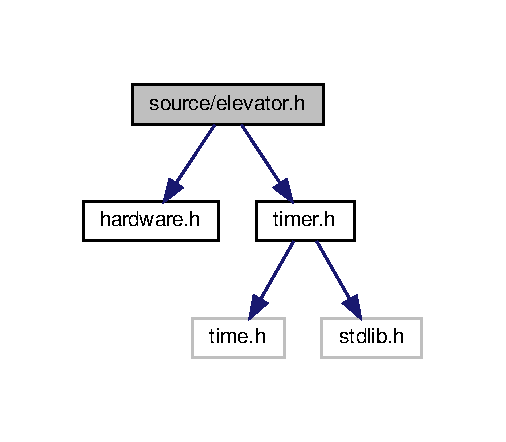
\includegraphics[width=243pt]{elevator_8h__incl}
\end{center}
\end{figure}
This graph shows which files directly or indirectly include this file\+:
\nopagebreak
\begin{figure}[H]
\begin{center}
\leavevmode
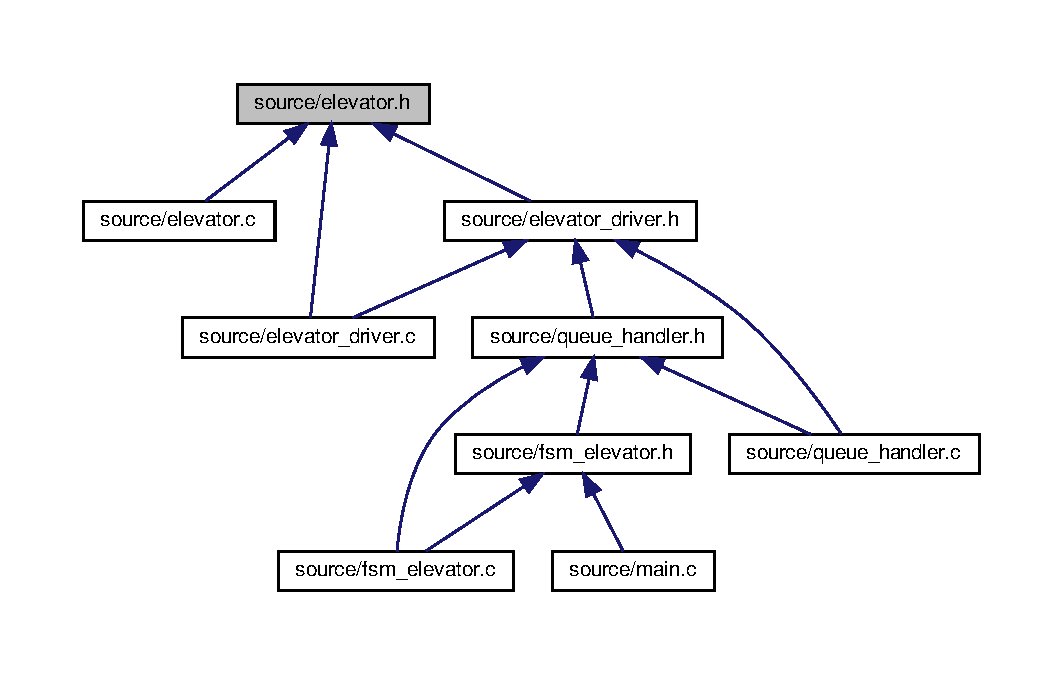
\includegraphics[width=350pt]{elevator_8h__dep__incl}
\end{center}
\end{figure}
\subsection*{Data Structures}
\begin{DoxyCompactItemize}
\item 
struct \hyperlink{structelevator__t}{elevator\+\_\+t}
\begin{DoxyCompactList}\small\item\em Struct that describes the elevator. It contains all the important variables for the process. \end{DoxyCompactList}\end{DoxyCompactItemize}
\subsection*{Macros}
\begin{DoxyCompactItemize}
\item 
\mbox{\Hypertarget{elevator_8h_a04e6314c901bd3977bcf0d5248744488}\label{elevator_8h_a04e6314c901bd3977bcf0d5248744488}} 
\#define {\bfseries O\+R\+D\+E\+R\+\_\+\+UP}~0
\item 
\mbox{\Hypertarget{elevator_8h_af84b377eeda4a2685049e86b29a70be5}\label{elevator_8h_af84b377eeda4a2685049e86b29a70be5}} 
\#define {\bfseries O\+R\+D\+E\+R\+\_\+\+D\+O\+WN}~1
\item 
\mbox{\Hypertarget{elevator_8h_a512aac99016300e247fe6a7610113c20}\label{elevator_8h_a512aac99016300e247fe6a7610113c20}} 
\#define {\bfseries O\+R\+D\+E\+R\+\_\+\+I\+N\+S\+I\+DE}~2
\item 
\mbox{\Hypertarget{elevator_8h_a737083ef6aae7fcbf7b755e0add99b16}\label{elevator_8h_a737083ef6aae7fcbf7b755e0add99b16}} 
\#define {\bfseries N\+U\+M\+B\+E\+R\+\_\+\+O\+F\+\_\+\+O\+R\+D\+E\+RS}~3
\item 
\mbox{\Hypertarget{elevator_8h_a00bda456521a6369be7f072fc4f43d59}\label{elevator_8h_a00bda456521a6369be7f072fc4f43d59}} 
\#define {\bfseries T\+O\+P\+\_\+\+F\+L\+O\+OR}~3
\item 
\mbox{\Hypertarget{elevator_8h_a360c832a52f523babde28630fe5561d3}\label{elevator_8h_a360c832a52f523babde28630fe5561d3}} 
\#define {\bfseries B\+O\+T\+T\+O\+M\+\_\+\+F\+L\+O\+OR}~0
\end{DoxyCompactItemize}
\subsection*{Enumerations}
\begin{DoxyCompactItemize}
\item 
\mbox{\Hypertarget{elevator_8h_a213dad15e4e24f653a4ac19140d9378a}\label{elevator_8h_a213dad15e4e24f653a4ac19140d9378a}} 
enum \hyperlink{elevator_8h_a213dad15e4e24f653a4ac19140d9378a}{elevator\+\_\+state\+\_\+t} \{ {\bfseries I\+D\+LE}, 
{\bfseries M\+O\+VE}, 
{\bfseries E\+M\+E\+R\+G\+E\+N\+C\+Y\+\_\+\+S\+T\+OP}, 
{\bfseries D\+O\+O\+R\+\_\+\+O\+P\+EN}
 \}\begin{DoxyCompactList}\small\item\em Enum used to define the different states of the elevator. \end{DoxyCompactList}
\end{DoxyCompactItemize}
\subsection*{Functions}
\begin{DoxyCompactItemize}
\item 
void \hyperlink{elevator_8h_a9b92734cb9648a7847c10238559bdd9d}{elevator\+\_\+lights} (\hyperlink{structelevator__t}{elevator\+\_\+t} $\ast$e)
\begin{DoxyCompactList}\small\item\em Function that controls all the lights in the elevator. \end{DoxyCompactList}\item 
void \hyperlink{elevator_8h_aa9ed29e4aeafe0cf248f52795a139160}{elevator\+\_\+clear\+\_\+all\+\_\+lights} ()
\begin{DoxyCompactList}\small\item\em Function that turns off all the outside and inside order lights. \end{DoxyCompactList}\end{DoxyCompactItemize}


\subsection{Detailed Description}
File that contains the elevator struct and basic elevator functions. 



\subsection{Function Documentation}
\mbox{\Hypertarget{elevator_8h_aa9ed29e4aeafe0cf248f52795a139160}\label{elevator_8h_aa9ed29e4aeafe0cf248f52795a139160}} 
\index{elevator.\+h@{elevator.\+h}!elevator\+\_\+clear\+\_\+all\+\_\+lights@{elevator\+\_\+clear\+\_\+all\+\_\+lights}}
\index{elevator\+\_\+clear\+\_\+all\+\_\+lights@{elevator\+\_\+clear\+\_\+all\+\_\+lights}!elevator.\+h@{elevator.\+h}}
\subsubsection{\texorpdfstring{elevator\+\_\+clear\+\_\+all\+\_\+lights()}{elevator\_clear\_all\_lights()}}
{\footnotesize\ttfamily void elevator\+\_\+clear\+\_\+all\+\_\+lights (\begin{DoxyParamCaption}{ }\end{DoxyParamCaption})}



Function that turns off all the outside and inside order lights. 


\begin{DoxyParams}{Parameters}
{\em \hyperlink{structelevator__t}{elevator\+\_\+t}} & $\ast$e, pointer to a struct that contains all the information important for running the elevator. \\
\hline
\end{DoxyParams}


Definition at line 51 of file elevator.\+c.

\mbox{\Hypertarget{elevator_8h_a9b92734cb9648a7847c10238559bdd9d}\label{elevator_8h_a9b92734cb9648a7847c10238559bdd9d}} 
\index{elevator.\+h@{elevator.\+h}!elevator\+\_\+lights@{elevator\+\_\+lights}}
\index{elevator\+\_\+lights@{elevator\+\_\+lights}!elevator.\+h@{elevator.\+h}}
\subsubsection{\texorpdfstring{elevator\+\_\+lights()}{elevator\_lights()}}
{\footnotesize\ttfamily void elevator\+\_\+lights (\begin{DoxyParamCaption}\item[{\hyperlink{structelevator__t}{elevator\+\_\+t} $\ast$}]{e }\end{DoxyParamCaption})}



Function that controls all the lights in the elevator. 

The function consist of a for loop that checks the order matrix and turns on the light is there is a order. It also turns on the stop light when the stop button is pushed. 
\begin{DoxyParams}{Parameters}
{\em \hyperlink{structelevator__t}{elevator\+\_\+t}} & $\ast$e, pointer to a struct that contains all the information important for running the elevator. \\
\hline
\end{DoxyParams}


Definition at line 6 of file elevator.\+c.


\hypertarget{elevator__driver_8h}{}\section{source/elevator\+\_\+driver.h File Reference}
\label{elevator__driver_8h}\index{source/elevator\+\_\+driver.\+h@{source/elevator\+\_\+driver.\+h}}


File that contains the functions needed for driving the elevator and getting information from the differnt sensors to upfate the floor.  


{\ttfamily \#include \char`\"{}elevator.\+h\char`\"{}}\newline
Include dependency graph for elevator\+\_\+driver.\+h\+:\nopagebreak
\begin{figure}[H]
\begin{center}
\leavevmode
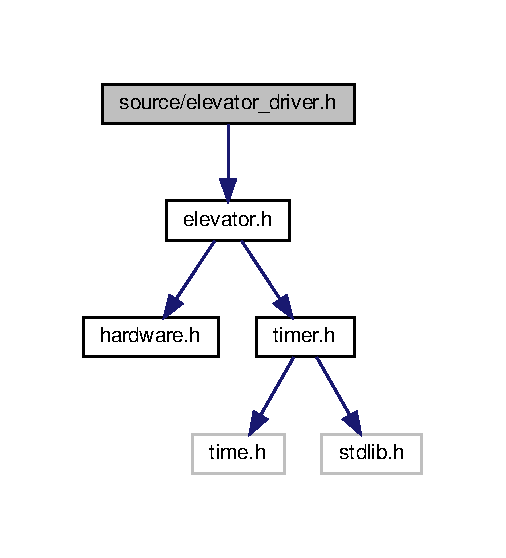
\includegraphics[width=243pt]{elevator__driver_8h__incl}
\end{center}
\end{figure}
This graph shows which files directly or indirectly include this file\+:\nopagebreak
\begin{figure}[H]
\begin{center}
\leavevmode
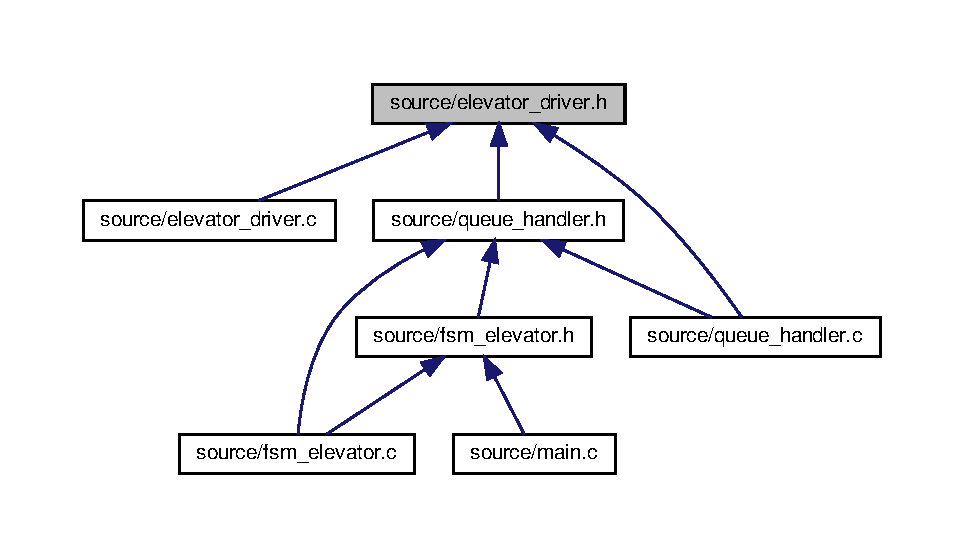
\includegraphics[width=350pt]{elevator__driver_8h__dep__incl}
\end{center}
\end{figure}
\subsection*{Macros}
\begin{DoxyCompactItemize}
\item 
\mbox{\Hypertarget{elevator__driver_8h_a5c5dcc1312c6767c2960b9bd15d4d80d}\label{elevator__driver_8h_a5c5dcc1312c6767c2960b9bd15d4d80d}} 
\#define {\bfseries D\+E\+F\+A\+U\+L\+T\+\_\+\+F\+L\+O\+OR}~0
\item 
\mbox{\Hypertarget{elevator__driver_8h_aa8cecfc5c5c054d2875c03e77b7be15d}\label{elevator__driver_8h_aa8cecfc5c5c054d2875c03e77b7be15d}} 
\#define {\bfseries T\+R\+UE}~1
\item 
\mbox{\Hypertarget{elevator__driver_8h_aa93f0eb578d23995850d61f7d61c55c1}\label{elevator__driver_8h_aa93f0eb578d23995850d61f7d61c55c1}} 
\#define {\bfseries F\+A\+L\+SE}~0
\end{DoxyCompactItemize}
\subsection*{Functions}
\begin{DoxyCompactItemize}
\item 
\mbox{\Hypertarget{elevator__driver_8h_a4de343ff2c5827e8bf59e63631420d71}\label{elevator__driver_8h_a4de343ff2c5827e8bf59e63631420d71}} 
void \hyperlink{elevator__driver_8h_a4de343ff2c5827e8bf59e63631420d71}{elevator\+\_\+driver\+\_\+stop} ()
\begin{DoxyCompactList}\small\item\em Function that stops the elevator when called. \end{DoxyCompactList}\item 
\mbox{\Hypertarget{elevator__driver_8h_a93852d87e388c89fcd8f4f4e7c7e39ba}\label{elevator__driver_8h_a93852d87e388c89fcd8f4f4e7c7e39ba}} 
void \hyperlink{elevator__driver_8h_a93852d87e388c89fcd8f4f4e7c7e39ba}{elevator\+\_\+driver\+\_\+default\+\_\+floor} (\hyperlink{structelevator__t}{elevator\+\_\+t} $\ast$e)
\begin{DoxyCompactList}\small\item\em Function that makes the elvator go to the initial floor, 1 atm. Used before the other functions when starting the elevator. \end{DoxyCompactList}\item 
\mbox{\Hypertarget{elevator__driver_8h_a149559f37920e54d8ccb75fd40100570}\label{elevator__driver_8h_a149559f37920e54d8ccb75fd40100570}} 
void \hyperlink{elevator__driver_8h_a149559f37920e54d8ccb75fd40100570}{elevator\+\_\+driver\+\_\+floor\+\_\+passed} (\hyperlink{structelevator__t}{elevator\+\_\+t} $\ast$e)
\begin{DoxyCompactList}\small\item\em Function that changes the last\+\_\+floor variable in the elevator struct to the last floor passed by the elevator. \end{DoxyCompactList}\item 
\mbox{\Hypertarget{elevator__driver_8h_a307e4b8bd67527bb6e0d012a47105caf}\label{elevator__driver_8h_a307e4b8bd67527bb6e0d012a47105caf}} 
int \hyperlink{elevator__driver_8h_a307e4b8bd67527bb6e0d012a47105caf}{elevator\+\_\+driver\+\_\+at\+\_\+floor} (\hyperlink{structelevator__t}{elevator\+\_\+t} $\ast$e)
\begin{DoxyCompactList}\small\item\em Function that returns 1 if the elevator is at a floor. Used when deciding to open the doors or not. \end{DoxyCompactList}\item 
\mbox{\Hypertarget{elevator__driver_8h_ad3b77f2b0f5eaa8f31a4d997d66a38d6}\label{elevator__driver_8h_ad3b77f2b0f5eaa8f31a4d997d66a38d6}} 
void \hyperlink{elevator__driver_8h_ad3b77f2b0f5eaa8f31a4d997d66a38d6}{elevator\+\_\+driver\+\_\+initialize\+\_\+elevator} (\hyperlink{structelevator__t}{elevator\+\_\+t} $\ast$e)
\begin{DoxyCompactList}\small\item\em Function that initializes the variables in the elevator. \end{DoxyCompactList}\item 
\mbox{\Hypertarget{elevator__driver_8h_ae0c3fece3603c485ddafc4e4da0827ce}\label{elevator__driver_8h_ae0c3fece3603c485ddafc4e4da0827ce}} 
void \hyperlink{elevator__driver_8h_ae0c3fece3603c485ddafc4e4da0827ce}{elevator\+\_\+driver\+\_\+range\+\_\+control} ()
\begin{DoxyCompactList}\small\item\em Function that stops the elevator if its on its way passed floor number 1 and 4. \end{DoxyCompactList}\end{DoxyCompactItemize}


\subsection{Detailed Description}
File that contains the functions needed for driving the elevator and getting information from the differnt sensors to upfate the floor. 


\hypertarget{fsm__elevator_8h}{}\section{source/fsm\+\_\+elevator.h File Reference}
\label{fsm__elevator_8h}\index{source/fsm\+\_\+elevator.\+h@{source/fsm\+\_\+elevator.\+h}}


File that contains the functions deciding what the elevator should do in the differnt states.  


{\ttfamily \#include \char`\"{}queue\+\_\+handler.\+h\char`\"{}}\newline
Include dependency graph for fsm\+\_\+elevator.\+h\+:\nopagebreak
\begin{figure}[H]
\begin{center}
\leavevmode
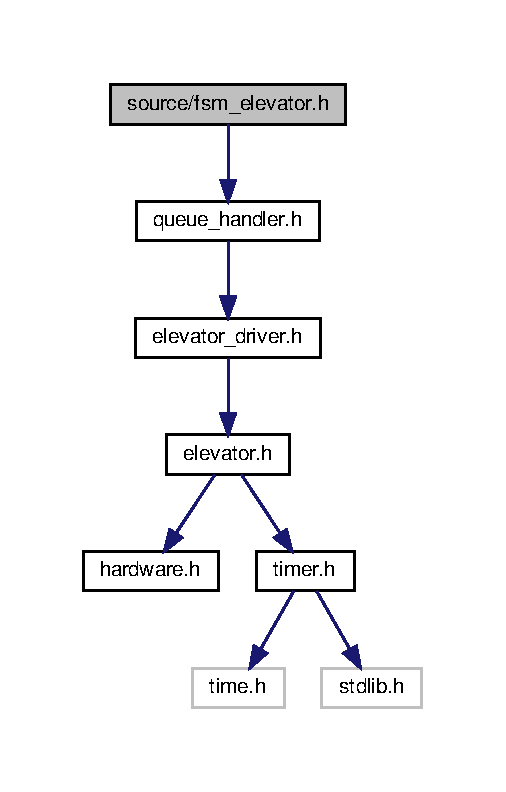
\includegraphics[width=243pt]{fsm__elevator_8h__incl}
\end{center}
\end{figure}
This graph shows which files directly or indirectly include this file\+:\nopagebreak
\begin{figure}[H]
\begin{center}
\leavevmode
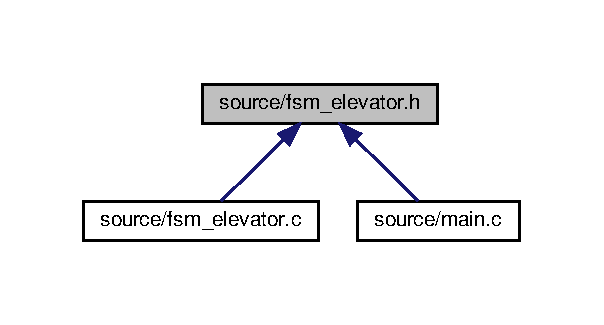
\includegraphics[width=290pt]{fsm__elevator_8h__dep__incl}
\end{center}
\end{figure}
\subsection*{Functions}
\begin{DoxyCompactItemize}
\item 
void \hyperlink{fsm__elevator_8h_a25d4b048860c891b45eefa2df09e2da6}{move\+\_\+state} (\hyperlink{structelevator__t}{elevator\+\_\+t} $\ast$e)
\begin{DoxyCompactList}\small\item\em Function that takes care of everything happening while the elevator is in M\+O\+VE state. \end{DoxyCompactList}\item 
void \hyperlink{fsm__elevator_8h_ab18323d0d8288582b3a604b64ba1700f}{idle\+\_\+state} (\hyperlink{structelevator__t}{elevator\+\_\+t} $\ast$e)
\begin{DoxyCompactList}\small\item\em Function that takes care of everything happening while the elevator is in I\+D\+LE state. \end{DoxyCompactList}\item 
void \hyperlink{fsm__elevator_8h_a6e1c7bfb2d29d318759dc12bcc46534a}{emergency\+\_\+stop\+\_\+state} (\hyperlink{structelevator__t}{elevator\+\_\+t} $\ast$e)
\begin{DoxyCompactList}\small\item\em Function that takes care of everything happening while the elevator is in E\+M\+E\+R\+G\+E\+N\+C\+Y\+\_\+\+S\+T\+OP state. \end{DoxyCompactList}\item 
void \hyperlink{fsm__elevator_8h_a3bd95f1165ffc670e1cfd6ac2b929b5a}{door\+\_\+state} (\hyperlink{structelevator__t}{elevator\+\_\+t} $\ast$e)
\begin{DoxyCompactList}\small\item\em Function that takes care of everything happening while the elevator is in D\+O\+O\+R\+\_\+\+O\+P\+EN state. \end{DoxyCompactList}\item 
void \hyperlink{fsm__elevator_8h_ab26d93b93ea5f0fb39c3c132f3bdd5e1}{fsm\+\_\+elevator\+\_\+go} (\hyperlink{structelevator__t}{elevator\+\_\+t} $\ast$e)
\begin{DoxyCompactList}\small\item\em The main fsm function that makes the elevator work. It contains a switch and switches between the differnt functions according to the elevators current state. \end{DoxyCompactList}\end{DoxyCompactItemize}


\subsection{Detailed Description}
File that contains the functions deciding what the elevator should do in the differnt states. 



\subsection{Function Documentation}
\mbox{\Hypertarget{fsm__elevator_8h_a3bd95f1165ffc670e1cfd6ac2b929b5a}\label{fsm__elevator_8h_a3bd95f1165ffc670e1cfd6ac2b929b5a}} 
\index{fsm\+\_\+elevator.\+h@{fsm\+\_\+elevator.\+h}!door\+\_\+state@{door\+\_\+state}}
\index{door\+\_\+state@{door\+\_\+state}!fsm\+\_\+elevator.\+h@{fsm\+\_\+elevator.\+h}}
\subsubsection{\texorpdfstring{door\+\_\+state()}{door\_state()}}
{\footnotesize\ttfamily void door\+\_\+state (\begin{DoxyParamCaption}\item[{\hyperlink{structelevator__t}{elevator\+\_\+t} $\ast$}]{e }\end{DoxyParamCaption})}



Function that takes care of everything happening while the elevator is in D\+O\+O\+R\+\_\+\+O\+P\+EN state. 


\begin{DoxyParams}{Parameters}
{\em \hyperlink{structelevator__t}{elevator\+\_\+t}} & Struct that contains all the information important for running the elevator. \\
\hline
\end{DoxyParams}


Definition at line 99 of file fsm\+\_\+elevator.\+c.

\mbox{\Hypertarget{fsm__elevator_8h_a6e1c7bfb2d29d318759dc12bcc46534a}\label{fsm__elevator_8h_a6e1c7bfb2d29d318759dc12bcc46534a}} 
\index{fsm\+\_\+elevator.\+h@{fsm\+\_\+elevator.\+h}!emergency\+\_\+stop\+\_\+state@{emergency\+\_\+stop\+\_\+state}}
\index{emergency\+\_\+stop\+\_\+state@{emergency\+\_\+stop\+\_\+state}!fsm\+\_\+elevator.\+h@{fsm\+\_\+elevator.\+h}}
\subsubsection{\texorpdfstring{emergency\+\_\+stop\+\_\+state()}{emergency\_stop\_state()}}
{\footnotesize\ttfamily void emergency\+\_\+stop\+\_\+state (\begin{DoxyParamCaption}\item[{\hyperlink{structelevator__t}{elevator\+\_\+t} $\ast$}]{e }\end{DoxyParamCaption})}



Function that takes care of everything happening while the elevator is in E\+M\+E\+R\+G\+E\+N\+C\+Y\+\_\+\+S\+T\+OP state. 


\begin{DoxyParams}{Parameters}
{\em \hyperlink{structelevator__t}{elevator\+\_\+t}} & Struct that contains all the information important for running the elevator. \\
\hline
\end{DoxyParams}


Definition at line 119 of file fsm\+\_\+elevator.\+c.

\mbox{\Hypertarget{fsm__elevator_8h_ab26d93b93ea5f0fb39c3c132f3bdd5e1}\label{fsm__elevator_8h_ab26d93b93ea5f0fb39c3c132f3bdd5e1}} 
\index{fsm\+\_\+elevator.\+h@{fsm\+\_\+elevator.\+h}!fsm\+\_\+elevator\+\_\+go@{fsm\+\_\+elevator\+\_\+go}}
\index{fsm\+\_\+elevator\+\_\+go@{fsm\+\_\+elevator\+\_\+go}!fsm\+\_\+elevator.\+h@{fsm\+\_\+elevator.\+h}}
\subsubsection{\texorpdfstring{fsm\+\_\+elevator\+\_\+go()}{fsm\_elevator\_go()}}
{\footnotesize\ttfamily void fsm\+\_\+elevator\+\_\+go (\begin{DoxyParamCaption}\item[{\hyperlink{structelevator__t}{elevator\+\_\+t} $\ast$}]{e }\end{DoxyParamCaption})}



The main fsm function that makes the elevator work. It contains a switch and switches between the differnt functions according to the elevators current state. 


\begin{DoxyItemize}
\item 
\begin{DoxyParams}{Parameters}
{\em \hyperlink{structelevator__t}{elevator\+\_\+t}} & Struct that contains all the information important for running the elevator. \\
\hline
\end{DoxyParams}

\end{DoxyItemize}

Definition at line 9 of file fsm\+\_\+elevator.\+c.

\mbox{\Hypertarget{fsm__elevator_8h_ab18323d0d8288582b3a604b64ba1700f}\label{fsm__elevator_8h_ab18323d0d8288582b3a604b64ba1700f}} 
\index{fsm\+\_\+elevator.\+h@{fsm\+\_\+elevator.\+h}!idle\+\_\+state@{idle\+\_\+state}}
\index{idle\+\_\+state@{idle\+\_\+state}!fsm\+\_\+elevator.\+h@{fsm\+\_\+elevator.\+h}}
\subsubsection{\texorpdfstring{idle\+\_\+state()}{idle\_state()}}
{\footnotesize\ttfamily void idle\+\_\+state (\begin{DoxyParamCaption}\item[{\hyperlink{structelevator__t}{elevator\+\_\+t} $\ast$}]{e }\end{DoxyParamCaption})}



Function that takes care of everything happening while the elevator is in I\+D\+LE state. 


\begin{DoxyParams}{Parameters}
{\em \hyperlink{structelevator__t}{elevator\+\_\+t}} & Struct that contains all the information important for running the elevator. \\
\hline
\end{DoxyParams}


Definition at line 31 of file fsm\+\_\+elevator.\+c.

\mbox{\Hypertarget{fsm__elevator_8h_a25d4b048860c891b45eefa2df09e2da6}\label{fsm__elevator_8h_a25d4b048860c891b45eefa2df09e2da6}} 
\index{fsm\+\_\+elevator.\+h@{fsm\+\_\+elevator.\+h}!move\+\_\+state@{move\+\_\+state}}
\index{move\+\_\+state@{move\+\_\+state}!fsm\+\_\+elevator.\+h@{fsm\+\_\+elevator.\+h}}
\subsubsection{\texorpdfstring{move\+\_\+state()}{move\_state()}}
{\footnotesize\ttfamily void move\+\_\+state (\begin{DoxyParamCaption}\item[{\hyperlink{structelevator__t}{elevator\+\_\+t} $\ast$}]{e }\end{DoxyParamCaption})}



Function that takes care of everything happening while the elevator is in M\+O\+VE state. 


\begin{DoxyParams}{Parameters}
{\em \hyperlink{structelevator__t}{elevator\+\_\+t}} & Struct that contains all the information important for running the elevator. \\
\hline
\end{DoxyParams}


Definition at line 78 of file fsm\+\_\+elevator.\+c.


\hypertarget{hardware_8h}{}\section{source/hardware.h File Reference}
\label{hardware_8h}\index{source/hardware.\+h@{source/hardware.\+h}}


Driver for the elevator hardware.  


This graph shows which files directly or indirectly include this file\+:
\nopagebreak
\begin{figure}[H]
\begin{center}
\leavevmode
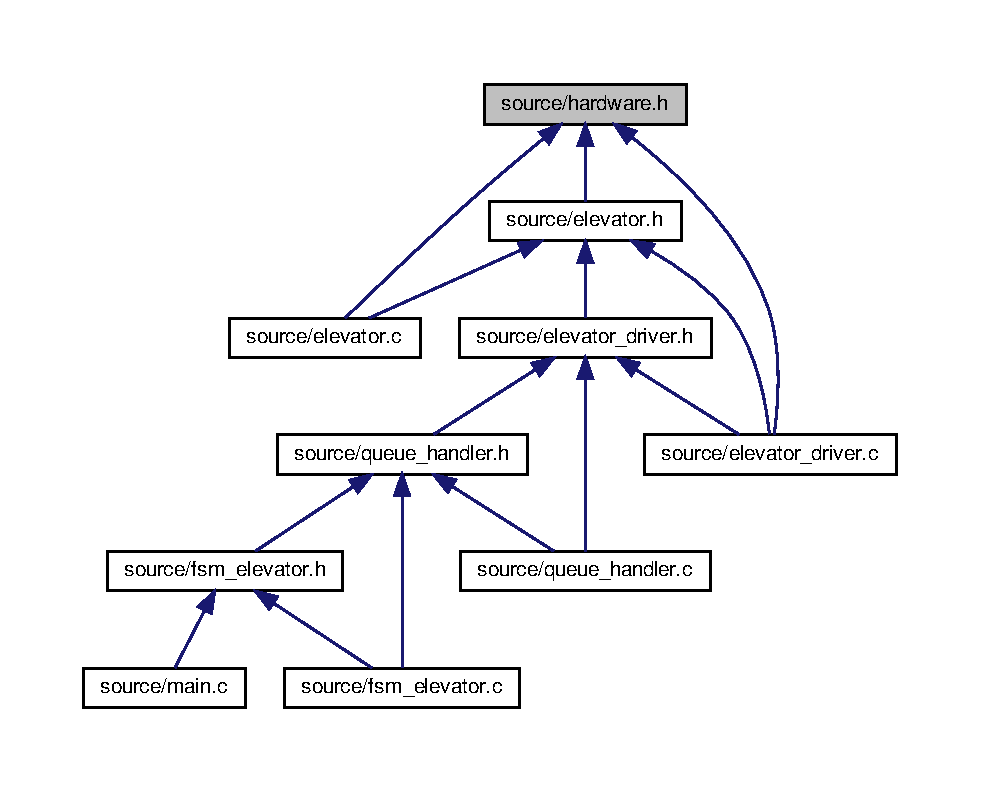
\includegraphics[width=350pt]{hardware_8h__dep__incl}
\end{center}
\end{figure}
\subsection*{Macros}
\begin{DoxyCompactItemize}
\item 
\mbox{\Hypertarget{hardware_8h_ae9e42615eade15633bd8c03b7a271a00}\label{hardware_8h_ae9e42615eade15633bd8c03b7a271a00}} 
\#define {\bfseries H\+A\+R\+D\+W\+A\+R\+E\+\_\+\+N\+U\+M\+B\+E\+R\+\_\+\+O\+F\+\_\+\+F\+L\+O\+O\+RS}~4
\end{DoxyCompactItemize}
\subsection*{Enumerations}
\begin{DoxyCompactItemize}
\item 
\mbox{\Hypertarget{hardware_8h_a2167c399a24df296afc432bcb88228af}\label{hardware_8h_a2167c399a24df296afc432bcb88228af}} 
enum \hyperlink{hardware_8h_a2167c399a24df296afc432bcb88228af}{Hardware\+Movement} \{ {\bfseries H\+A\+R\+D\+W\+A\+R\+E\+\_\+\+M\+O\+V\+E\+M\+E\+N\+T\+\_\+\+UP}, 
{\bfseries H\+A\+R\+D\+W\+A\+R\+E\+\_\+\+M\+O\+V\+E\+M\+E\+N\+T\+\_\+\+S\+T\+OP}, 
{\bfseries H\+A\+R\+D\+W\+A\+R\+E\+\_\+\+M\+O\+V\+E\+M\+E\+N\+T\+\_\+\+D\+O\+WN}
 \}\begin{DoxyCompactList}\small\item\em Movement type used in {\ttfamily hardware\+\_\+command\+\_\+movement}. \end{DoxyCompactList}
\item 
\mbox{\Hypertarget{hardware_8h_a796a8de8ce0ae769d7dbd3327a7bdbe7}\label{hardware_8h_a796a8de8ce0ae769d7dbd3327a7bdbe7}} 
enum \hyperlink{hardware_8h_a796a8de8ce0ae769d7dbd3327a7bdbe7}{Hardware\+Order} \{ {\bfseries H\+A\+R\+D\+W\+A\+R\+E\+\_\+\+O\+R\+D\+E\+R\+\_\+\+UP}, 
{\bfseries H\+A\+R\+D\+W\+A\+R\+E\+\_\+\+O\+R\+D\+E\+R\+\_\+\+I\+N\+S\+I\+DE}, 
{\bfseries H\+A\+R\+D\+W\+A\+R\+E\+\_\+\+O\+R\+D\+E\+R\+\_\+\+D\+O\+WN}
 \}\begin{DoxyCompactList}\small\item\em Order type used in {\ttfamily hardware\+\_\+read\+\_\+order} and in {\ttfamily hardware\+\_\+command\+\_\+order\+\_\+light}. \end{DoxyCompactList}
\end{DoxyCompactItemize}
\subsection*{Functions}
\begin{DoxyCompactItemize}
\item 
int \hyperlink{hardware_8h_a054b8fb8768311d46be58d6a4890d771}{hardware\+\_\+init} ()
\begin{DoxyCompactList}\small\item\em Initializes the elevator control hardware. Must be called once before other calls to the elevator hardware driver. \end{DoxyCompactList}\item 
void \hyperlink{hardware_8h_a01de081ef0510a111053c18cd31afa27}{hardware\+\_\+command\+\_\+movement} (\hyperlink{hardware_8h_a2167c399a24df296afc432bcb88228af}{Hardware\+Movement} movement)
\begin{DoxyCompactList}\small\item\em Commands the elevator to either move up or down, or commands it to halt. \end{DoxyCompactList}\item 
int \hyperlink{hardware_8h_a4a77b27c86675c00b513db3445966804}{hardware\+\_\+read\+\_\+stop\+\_\+signal} ()
\begin{DoxyCompactList}\small\item\em Polls the hardware for the current stop signal. \end{DoxyCompactList}\item 
int \hyperlink{hardware_8h_a459fe57a3ee4bc2a28e8a15b2ab14c2d}{hardware\+\_\+read\+\_\+obstruction\+\_\+signal} ()
\begin{DoxyCompactList}\small\item\em Polls the hardware for the current obstruction signal. \end{DoxyCompactList}\item 
int \hyperlink{hardware_8h_ab048489e6302bb5604aad753f2d7d501}{hardware\+\_\+read\+\_\+floor\+\_\+sensor} (int floor)
\begin{DoxyCompactList}\small\item\em Polls the floor sensor for the given {\ttfamily floor}. \end{DoxyCompactList}\item 
int \hyperlink{hardware_8h_a87917f3aa093fb46ca821a400d011ee8}{hardware\+\_\+read\+\_\+order} (int floor, \hyperlink{hardware_8h_a796a8de8ce0ae769d7dbd3327a7bdbe7}{Hardware\+Order} order\+\_\+type)
\begin{DoxyCompactList}\small\item\em Polls the hardware for the status of orders from floor {\ttfamily floor} of type {\ttfamily order\+\_\+type}. \end{DoxyCompactList}\item 
void \hyperlink{hardware_8h_a80d99ddaa8e7b58c9a88b60ea553c1b6}{hardware\+\_\+command\+\_\+door\+\_\+open} (int door\+\_\+open)
\begin{DoxyCompactList}\small\item\em Commands the hardware to open-\/ or close the elevator door. \end{DoxyCompactList}\item 
void \hyperlink{hardware_8h_a407a6ec035ba357de6aa0fbe55501d1e}{hardware\+\_\+command\+\_\+floor\+\_\+indicator\+\_\+on} (int floor)
\begin{DoxyCompactList}\small\item\em Commands the hardware to turn on the floor indicator for {\ttfamily floor}. All indicators all mutually exclusive; other indicator lights will turn off. \end{DoxyCompactList}\item 
void \hyperlink{hardware_8h_aa75b3ac17f72b25946414f48d0063a10}{hardware\+\_\+command\+\_\+stop\+\_\+light} (int on)
\begin{DoxyCompactList}\small\item\em Sets the light in the panel stop button. \end{DoxyCompactList}\item 
void \hyperlink{hardware_8h_aa9b33faa52f0ec5b614d3e7dc05be140}{hardware\+\_\+command\+\_\+order\+\_\+light} (int floor, \hyperlink{hardware_8h_a796a8de8ce0ae769d7dbd3327a7bdbe7}{Hardware\+Order} order\+\_\+type, int on)
\begin{DoxyCompactList}\small\item\em Sets the light in a button corresponding to an order of type {\ttfamily order\+\_\+type}, at floor {\ttfamily floor}. \end{DoxyCompactList}\end{DoxyCompactItemize}


\subsection{Detailed Description}
Driver for the elevator hardware. 

Neatly wraps up Martin Korsgaard\textquotesingle{}s spaghetti from 2006 ;)

Kolbjørn Austreng 

\subsection{Function Documentation}
\mbox{\Hypertarget{hardware_8h_a80d99ddaa8e7b58c9a88b60ea553c1b6}\label{hardware_8h_a80d99ddaa8e7b58c9a88b60ea553c1b6}} 
\index{hardware.\+h@{hardware.\+h}!hardware\+\_\+command\+\_\+door\+\_\+open@{hardware\+\_\+command\+\_\+door\+\_\+open}}
\index{hardware\+\_\+command\+\_\+door\+\_\+open@{hardware\+\_\+command\+\_\+door\+\_\+open}!hardware.\+h@{hardware.\+h}}
\subsubsection{\texorpdfstring{hardware\+\_\+command\+\_\+door\+\_\+open()}{hardware\_command\_door\_open()}}
{\footnotesize\ttfamily void hardware\+\_\+command\+\_\+door\+\_\+open (\begin{DoxyParamCaption}\item[{int}]{door\+\_\+open }\end{DoxyParamCaption})}



Commands the hardware to open-\/ or close the elevator door. 


\begin{DoxyParams}{Parameters}
{\em door\+\_\+open} & A truthy value (non-\/zero) to open the door; 0 to close. \\
\hline
\end{DoxyParams}
\mbox{\Hypertarget{hardware_8h_a407a6ec035ba357de6aa0fbe55501d1e}\label{hardware_8h_a407a6ec035ba357de6aa0fbe55501d1e}} 
\index{hardware.\+h@{hardware.\+h}!hardware\+\_\+command\+\_\+floor\+\_\+indicator\+\_\+on@{hardware\+\_\+command\+\_\+floor\+\_\+indicator\+\_\+on}}
\index{hardware\+\_\+command\+\_\+floor\+\_\+indicator\+\_\+on@{hardware\+\_\+command\+\_\+floor\+\_\+indicator\+\_\+on}!hardware.\+h@{hardware.\+h}}
\subsubsection{\texorpdfstring{hardware\+\_\+command\+\_\+floor\+\_\+indicator\+\_\+on()}{hardware\_command\_floor\_indicator\_on()}}
{\footnotesize\ttfamily void hardware\+\_\+command\+\_\+floor\+\_\+indicator\+\_\+on (\begin{DoxyParamCaption}\item[{int}]{floor }\end{DoxyParamCaption})}



Commands the hardware to turn on the floor indicator for {\ttfamily floor}. All indicators all mutually exclusive; other indicator lights will turn off. 


\begin{DoxyParams}{Parameters}
{\em floor} & Floor to turn on the indicator for.\\
\hline
\end{DoxyParams}
\begin{DoxyWarning}{Warning}
Owing to peculiarities in the hardware construction, there will always be one indicator active. 
\end{DoxyWarning}
\mbox{\Hypertarget{hardware_8h_a01de081ef0510a111053c18cd31afa27}\label{hardware_8h_a01de081ef0510a111053c18cd31afa27}} 
\index{hardware.\+h@{hardware.\+h}!hardware\+\_\+command\+\_\+movement@{hardware\+\_\+command\+\_\+movement}}
\index{hardware\+\_\+command\+\_\+movement@{hardware\+\_\+command\+\_\+movement}!hardware.\+h@{hardware.\+h}}
\subsubsection{\texorpdfstring{hardware\+\_\+command\+\_\+movement()}{hardware\_command\_movement()}}
{\footnotesize\ttfamily void hardware\+\_\+command\+\_\+movement (\begin{DoxyParamCaption}\item[{\hyperlink{hardware_8h_a2167c399a24df296afc432bcb88228af}{Hardware\+Movement}}]{movement }\end{DoxyParamCaption})}



Commands the elevator to either move up or down, or commands it to halt. 


\begin{DoxyParams}{Parameters}
{\em movement} & Commanded movement. \\
\hline
\end{DoxyParams}
\mbox{\Hypertarget{hardware_8h_aa9b33faa52f0ec5b614d3e7dc05be140}\label{hardware_8h_aa9b33faa52f0ec5b614d3e7dc05be140}} 
\index{hardware.\+h@{hardware.\+h}!hardware\+\_\+command\+\_\+order\+\_\+light@{hardware\+\_\+command\+\_\+order\+\_\+light}}
\index{hardware\+\_\+command\+\_\+order\+\_\+light@{hardware\+\_\+command\+\_\+order\+\_\+light}!hardware.\+h@{hardware.\+h}}
\subsubsection{\texorpdfstring{hardware\+\_\+command\+\_\+order\+\_\+light()}{hardware\_command\_order\_light()}}
{\footnotesize\ttfamily void hardware\+\_\+command\+\_\+order\+\_\+light (\begin{DoxyParamCaption}\item[{int}]{floor,  }\item[{\hyperlink{hardware_8h_a796a8de8ce0ae769d7dbd3327a7bdbe7}{Hardware\+Order}}]{order\+\_\+type,  }\item[{int}]{on }\end{DoxyParamCaption})}



Sets the light in a button corresponding to an order of type {\ttfamily order\+\_\+type}, at floor {\ttfamily floor}. 


\begin{DoxyParams}{Parameters}
{\em floor} & The floor of the order indicator. \\
\hline
{\em order\+\_\+type} & The type of order. \\
\hline
{\em on} & A truthy value (non-\/zero) to turn the light on; 0 to turn it off. \\
\hline
\end{DoxyParams}
\mbox{\Hypertarget{hardware_8h_aa75b3ac17f72b25946414f48d0063a10}\label{hardware_8h_aa75b3ac17f72b25946414f48d0063a10}} 
\index{hardware.\+h@{hardware.\+h}!hardware\+\_\+command\+\_\+stop\+\_\+light@{hardware\+\_\+command\+\_\+stop\+\_\+light}}
\index{hardware\+\_\+command\+\_\+stop\+\_\+light@{hardware\+\_\+command\+\_\+stop\+\_\+light}!hardware.\+h@{hardware.\+h}}
\subsubsection{\texorpdfstring{hardware\+\_\+command\+\_\+stop\+\_\+light()}{hardware\_command\_stop\_light()}}
{\footnotesize\ttfamily void hardware\+\_\+command\+\_\+stop\+\_\+light (\begin{DoxyParamCaption}\item[{int}]{on }\end{DoxyParamCaption})}



Sets the light in the panel stop button. 


\begin{DoxyParams}{Parameters}
{\em on} & A truthy value (non-\/zero) to turn the light on; 0 to turn it off. \\
\hline
\end{DoxyParams}
\mbox{\Hypertarget{hardware_8h_a054b8fb8768311d46be58d6a4890d771}\label{hardware_8h_a054b8fb8768311d46be58d6a4890d771}} 
\index{hardware.\+h@{hardware.\+h}!hardware\+\_\+init@{hardware\+\_\+init}}
\index{hardware\+\_\+init@{hardware\+\_\+init}!hardware.\+h@{hardware.\+h}}
\subsubsection{\texorpdfstring{hardware\+\_\+init()}{hardware\_init()}}
{\footnotesize\ttfamily int hardware\+\_\+init (\begin{DoxyParamCaption}{ }\end{DoxyParamCaption})}



Initializes the elevator control hardware. Must be called once before other calls to the elevator hardware driver. 

\begin{DoxyReturn}{Returns}
0 on success. Non-\/zero for failure. 
\end{DoxyReturn}
\mbox{\Hypertarget{hardware_8h_ab048489e6302bb5604aad753f2d7d501}\label{hardware_8h_ab048489e6302bb5604aad753f2d7d501}} 
\index{hardware.\+h@{hardware.\+h}!hardware\+\_\+read\+\_\+floor\+\_\+sensor@{hardware\+\_\+read\+\_\+floor\+\_\+sensor}}
\index{hardware\+\_\+read\+\_\+floor\+\_\+sensor@{hardware\+\_\+read\+\_\+floor\+\_\+sensor}!hardware.\+h@{hardware.\+h}}
\subsubsection{\texorpdfstring{hardware\+\_\+read\+\_\+floor\+\_\+sensor()}{hardware\_read\_floor\_sensor()}}
{\footnotesize\ttfamily int hardware\+\_\+read\+\_\+floor\+\_\+sensor (\begin{DoxyParamCaption}\item[{int}]{floor }\end{DoxyParamCaption})}



Polls the floor sensor for the given {\ttfamily floor}. 


\begin{DoxyParams}{Parameters}
{\em floor} & Inquired floor.\\
\hline
\end{DoxyParams}
\begin{DoxyReturn}{Returns}
1 if the elevator is at {\ttfamily floor}, otherwise 0; 
\end{DoxyReturn}
\mbox{\Hypertarget{hardware_8h_a459fe57a3ee4bc2a28e8a15b2ab14c2d}\label{hardware_8h_a459fe57a3ee4bc2a28e8a15b2ab14c2d}} 
\index{hardware.\+h@{hardware.\+h}!hardware\+\_\+read\+\_\+obstruction\+\_\+signal@{hardware\+\_\+read\+\_\+obstruction\+\_\+signal}}
\index{hardware\+\_\+read\+\_\+obstruction\+\_\+signal@{hardware\+\_\+read\+\_\+obstruction\+\_\+signal}!hardware.\+h@{hardware.\+h}}
\subsubsection{\texorpdfstring{hardware\+\_\+read\+\_\+obstruction\+\_\+signal()}{hardware\_read\_obstruction\_signal()}}
{\footnotesize\ttfamily int hardware\+\_\+read\+\_\+obstruction\+\_\+signal (\begin{DoxyParamCaption}{ }\end{DoxyParamCaption})}



Polls the hardware for the current obstruction signal. 

\begin{DoxyReturn}{Returns}
1 if the obstruction signal is high; 0 if it is low. 
\end{DoxyReturn}
\mbox{\Hypertarget{hardware_8h_a87917f3aa093fb46ca821a400d011ee8}\label{hardware_8h_a87917f3aa093fb46ca821a400d011ee8}} 
\index{hardware.\+h@{hardware.\+h}!hardware\+\_\+read\+\_\+order@{hardware\+\_\+read\+\_\+order}}
\index{hardware\+\_\+read\+\_\+order@{hardware\+\_\+read\+\_\+order}!hardware.\+h@{hardware.\+h}}
\subsubsection{\texorpdfstring{hardware\+\_\+read\+\_\+order()}{hardware\_read\_order()}}
{\footnotesize\ttfamily int hardware\+\_\+read\+\_\+order (\begin{DoxyParamCaption}\item[{int}]{floor,  }\item[{\hyperlink{hardware_8h_a796a8de8ce0ae769d7dbd3327a7bdbe7}{Hardware\+Order}}]{order\+\_\+type }\end{DoxyParamCaption})}



Polls the hardware for the status of orders from floor {\ttfamily floor} of type {\ttfamily order\+\_\+type}. 


\begin{DoxyParams}{Parameters}
{\em floor} & Inquired floor. \\
\hline
{\em order\+\_\+type} & \\
\hline
\end{DoxyParams}
\begin{DoxyReturn}{Returns}
1 if the combination of {\ttfamily floor} and {\ttfamily order\+\_\+type} is being requested, otherwise 0. 
\end{DoxyReturn}
\mbox{\Hypertarget{hardware_8h_a4a77b27c86675c00b513db3445966804}\label{hardware_8h_a4a77b27c86675c00b513db3445966804}} 
\index{hardware.\+h@{hardware.\+h}!hardware\+\_\+read\+\_\+stop\+\_\+signal@{hardware\+\_\+read\+\_\+stop\+\_\+signal}}
\index{hardware\+\_\+read\+\_\+stop\+\_\+signal@{hardware\+\_\+read\+\_\+stop\+\_\+signal}!hardware.\+h@{hardware.\+h}}
\subsubsection{\texorpdfstring{hardware\+\_\+read\+\_\+stop\+\_\+signal()}{hardware\_read\_stop\_signal()}}
{\footnotesize\ttfamily int hardware\+\_\+read\+\_\+stop\+\_\+signal (\begin{DoxyParamCaption}{ }\end{DoxyParamCaption})}



Polls the hardware for the current stop signal. 

\begin{DoxyReturn}{Returns}
1 if the stop signal is high; 0 if it is low. 
\end{DoxyReturn}

\hypertarget{queue__handler_8h}{}\section{source/queue\+\_\+handler.h File Reference}
\label{queue__handler_8h}\index{source/queue\+\_\+handler.\+h@{source/queue\+\_\+handler.\+h}}


Function that contains all the different operations performed on the queue matrix.  


{\ttfamily \#include \char`\"{}elevator\+\_\+driver.\+h\char`\"{}}\newline
Include dependency graph for queue\+\_\+handler.\+h\+:\nopagebreak
\begin{figure}[H]
\begin{center}
\leavevmode
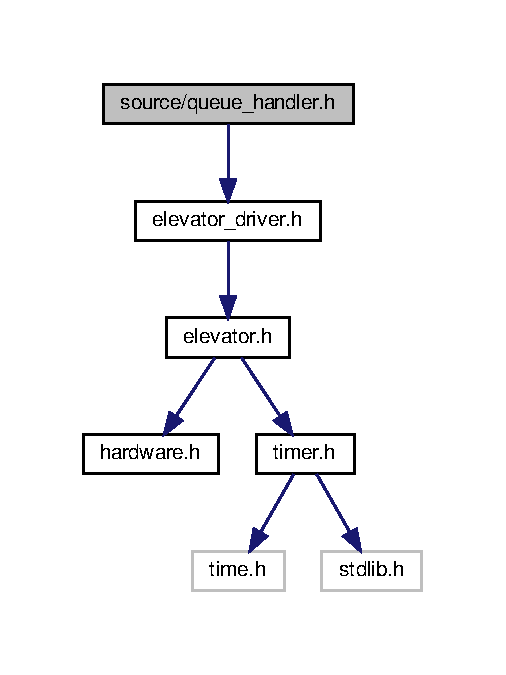
\includegraphics[width=243pt]{queue__handler_8h__incl}
\end{center}
\end{figure}
This graph shows which files directly or indirectly include this file\+:\nopagebreak
\begin{figure}[H]
\begin{center}
\leavevmode
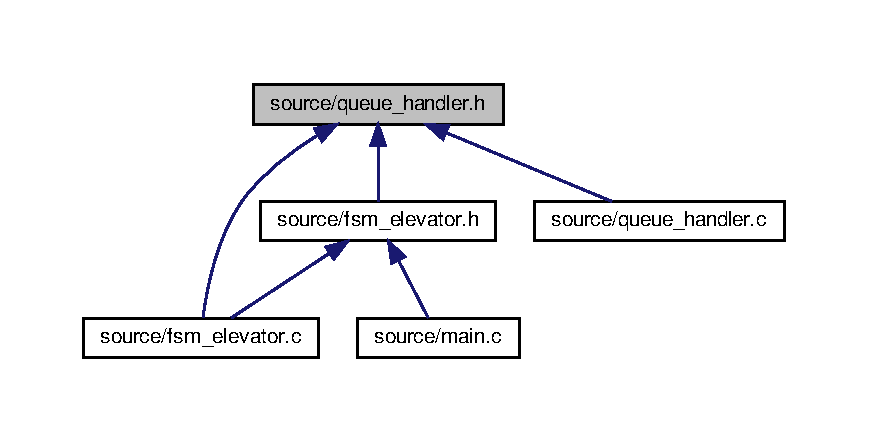
\includegraphics[width=350pt]{queue__handler_8h__dep__incl}
\end{center}
\end{figure}
\subsection*{Macros}
\begin{DoxyCompactItemize}
\item 
\mbox{\Hypertarget{queue__handler_8h_aa8cecfc5c5c054d2875c03e77b7be15d}\label{queue__handler_8h_aa8cecfc5c5c054d2875c03e77b7be15d}} 
\#define {\bfseries T\+R\+UE}~1
\item 
\mbox{\Hypertarget{queue__handler_8h_aa93f0eb578d23995850d61f7d61c55c1}\label{queue__handler_8h_aa93f0eb578d23995850d61f7d61c55c1}} 
\#define {\bfseries F\+A\+L\+SE}~0
\end{DoxyCompactItemize}
\subsection*{Functions}
\begin{DoxyCompactItemize}
\item 
void \hyperlink{queue__handler_8h_ae5d2620687480f2b74abf412586cc496}{queue\+\_\+handler\+\_\+clear\+\_\+queue} (\hyperlink{structelevator__t}{elevator\+\_\+t} $\ast$e)
\begin{DoxyCompactList}\small\item\em Function that clears the queue matrix in case of emergency stop while moving. \end{DoxyCompactList}\item 
void \hyperlink{queue__handler_8h_a185d3676b58fa2736cc0be19d22d7e30}{queue\+\_\+handler\+\_\+update\+\_\+queue\+\_\+outside} (\hyperlink{structelevator__t}{elevator\+\_\+t} $\ast$e)
\begin{DoxyCompactList}\small\item\em Function that searches for orders and updates the queue. \end{DoxyCompactList}\item 
int \hyperlink{queue__handler_8h_ac05310be57c5b344e7a47437cd86b99b}{queue\+\_\+handler\+\_\+change\+\_\+dir} (\hyperlink{structelevator__t}{elevator\+\_\+t} $\ast$e)
\begin{DoxyCompactList}\small\item\em Function that changes the current direction the the elevator. \end{DoxyCompactList}\item 
void \hyperlink{queue__handler_8h_ab4637cd308b26a882949b7a018822a81}{queue\+\_\+handler\+\_\+order\+\_\+complete} (\hyperlink{structelevator__t}{elevator\+\_\+t} $\ast$e)
\begin{DoxyCompactList}\small\item\em Function that changes the number in the queue from 1 to 0 after an order is complete. \end{DoxyCompactList}\item 
void \hyperlink{queue__handler_8h_acf89f0770228e9bd558d6314ec4c2aed}{queue\+\_\+handler\+\_\+update\+\_\+queue\+\_\+inside} (\hyperlink{structelevator__t}{elevator\+\_\+t} $\ast$e)
\begin{DoxyCompactList}\small\item\em Function that searches for orders from inside the elevator and updates the queue matrix if any orders. \end{DoxyCompactList}\item 
int \hyperlink{queue__handler_8h_a268a7a574af150a80c54ba8725315875}{queue\+\_\+handler\+\_\+stop} (\hyperlink{structelevator__t}{elevator\+\_\+t} $\ast$e)
\begin{DoxyCompactList}\small\item\em Function that returns 1 if the elevator should stop at current floor, and 0 if not. \end{DoxyCompactList}\item 
int \hyperlink{queue__handler_8h_aade312fd5d8424ebd3967f9e75473a6f}{queue\+\_\+handler\+\_\+order\+\_\+at\+\_\+current\+\_\+floor} (\hyperlink{structelevator__t}{elevator\+\_\+t} $\ast$e)
\begin{DoxyCompactList}\small\item\em Function that checks if there is an order of any type at the current floor. \end{DoxyCompactList}\item 
int \hyperlink{queue__handler_8h_af5c0f9018cafb915e72da3aad556684e}{queue\+\_\+handler\+\_\+emergency} (\hyperlink{structelevator__t}{elevator\+\_\+t} $\ast$e)
\begin{DoxyCompactList}\small\item\em Function for chosing the next direction for the elevator when the elevator is between floors in emergency state. \end{DoxyCompactList}\item 
int \hyperlink{queue__handler_8h_a4d8004bb433b559e61cea614ac3b2ce2}{queue\+\_\+handler\+\_\+pass\+\_\+floor} (\hyperlink{structelevator__t}{elevator\+\_\+t} $\ast$e)
\begin{DoxyCompactList}\small\item\em Function that decides if the elevator should pass a floor due to orders above or not. \end{DoxyCompactList}\item 
int \hyperlink{queue__handler_8h_a6cea3d2867bde86ca19de6b6aec905ca}{queue\+\_\+handler\+\_\+order\+\_\+above} (\hyperlink{structelevator__t}{elevator\+\_\+t} $\ast$e)
\begin{DoxyCompactList}\small\item\em Function that iterates through the above floors and searches for orders of any type. \end{DoxyCompactList}\item 
int \hyperlink{queue__handler_8h_a8f6f1c58428646fa957d97d9b1656a30}{queue\+\_\+handler\+\_\+order\+\_\+below} (\hyperlink{structelevator__t}{elevator\+\_\+t} $\ast$e)
\begin{DoxyCompactList}\small\item\em Function that iterates through the below floors and searches for orders of any type. \end{DoxyCompactList}\end{DoxyCompactItemize}


\subsection{Detailed Description}
Function that contains all the different operations performed on the queue matrix. 

\begin{DoxyAuthor}{Author}
your name (\href{mailto:you@domain.com}{\tt you@domain.\+com}) 
\end{DoxyAuthor}


\subsection{Function Documentation}
\mbox{\Hypertarget{queue__handler_8h_ac05310be57c5b344e7a47437cd86b99b}\label{queue__handler_8h_ac05310be57c5b344e7a47437cd86b99b}} 
\index{queue\+\_\+handler.\+h@{queue\+\_\+handler.\+h}!queue\+\_\+handler\+\_\+change\+\_\+dir@{queue\+\_\+handler\+\_\+change\+\_\+dir}}
\index{queue\+\_\+handler\+\_\+change\+\_\+dir@{queue\+\_\+handler\+\_\+change\+\_\+dir}!queue\+\_\+handler.\+h@{queue\+\_\+handler.\+h}}
\subsubsection{\texorpdfstring{queue\+\_\+handler\+\_\+change\+\_\+dir()}{queue\_handler\_change\_dir()}}
{\footnotesize\ttfamily int queue\+\_\+handler\+\_\+change\+\_\+dir (\begin{DoxyParamCaption}\item[{\hyperlink{structelevator__t}{elevator\+\_\+t} $\ast$}]{e }\end{DoxyParamCaption})}



Function that changes the current direction the the elevator. 

If current direction is up, the function will first search for orders above before searching for orders below afterwards. Likewise, if current direction is down, the functtion first search for orders below, before searching for orders above. When the elevator is in idle state it will switch between searching for orders above and below and return 1 as long as no order is found. When an order is found it wil return 0. This means that as long as the elevator returns 1 it has not found an order. 
\begin{DoxyParams}{Parameters}
{\em \hyperlink{structelevator__t}{elevator\+\_\+t}} & Struct that contains all the information important for running the elevator. \\
\hline
\end{DoxyParams}
\begin{DoxyReturn}{Returns}
1 if the elevator should change direction and 0 if not. 
\end{DoxyReturn}


Definition at line 51 of file queue\+\_\+handler.\+c.

\mbox{\Hypertarget{queue__handler_8h_ae5d2620687480f2b74abf412586cc496}\label{queue__handler_8h_ae5d2620687480f2b74abf412586cc496}} 
\index{queue\+\_\+handler.\+h@{queue\+\_\+handler.\+h}!queue\+\_\+handler\+\_\+clear\+\_\+queue@{queue\+\_\+handler\+\_\+clear\+\_\+queue}}
\index{queue\+\_\+handler\+\_\+clear\+\_\+queue@{queue\+\_\+handler\+\_\+clear\+\_\+queue}!queue\+\_\+handler.\+h@{queue\+\_\+handler.\+h}}
\subsubsection{\texorpdfstring{queue\+\_\+handler\+\_\+clear\+\_\+queue()}{queue\_handler\_clear\_queue()}}
{\footnotesize\ttfamily void queue\+\_\+handler\+\_\+clear\+\_\+queue (\begin{DoxyParamCaption}\item[{\hyperlink{structelevator__t}{elevator\+\_\+t} $\ast$}]{e }\end{DoxyParamCaption})}



Function that clears the queue matrix in case of emergency stop while moving. 


\begin{DoxyParams}{Parameters}
{\em \hyperlink{structelevator__t}{elevator\+\_\+t}} & Struct that contains all the information important for running the elevator. \\
\hline
\end{DoxyParams}


Definition at line 6 of file queue\+\_\+handler.\+c.

\mbox{\Hypertarget{queue__handler_8h_af5c0f9018cafb915e72da3aad556684e}\label{queue__handler_8h_af5c0f9018cafb915e72da3aad556684e}} 
\index{queue\+\_\+handler.\+h@{queue\+\_\+handler.\+h}!queue\+\_\+handler\+\_\+emergency@{queue\+\_\+handler\+\_\+emergency}}
\index{queue\+\_\+handler\+\_\+emergency@{queue\+\_\+handler\+\_\+emergency}!queue\+\_\+handler.\+h@{queue\+\_\+handler.\+h}}
\subsubsection{\texorpdfstring{queue\+\_\+handler\+\_\+emergency()}{queue\_handler\_emergency()}}
{\footnotesize\ttfamily int queue\+\_\+handler\+\_\+emergency (\begin{DoxyParamCaption}\item[{\hyperlink{structelevator__t}{elevator\+\_\+t} $\ast$}]{e }\end{DoxyParamCaption})}



Function for chosing the next direction for the elevator when the elevator is between floors in emergency state. 

If the elevator stops between floors we need to have a differnt function to choose direction. For example if we are between the first and second floor with current direction upwards and an order is made in the first floor, the elevator does not know it is between floors and not at the first floor, as the variable current\+\_\+floor says. Therefore the functtion needs to change the current floor from first to second and also change current direction to down. The same applies to other direction and floors.

\begin{DoxyReturn}{Returns}
1 if direction and floor is set as it should, and 0 otherwise. 
\end{DoxyReturn}


Definition at line 97 of file queue\+\_\+handler.\+c.

\mbox{\Hypertarget{queue__handler_8h_a6cea3d2867bde86ca19de6b6aec905ca}\label{queue__handler_8h_a6cea3d2867bde86ca19de6b6aec905ca}} 
\index{queue\+\_\+handler.\+h@{queue\+\_\+handler.\+h}!queue\+\_\+handler\+\_\+order\+\_\+above@{queue\+\_\+handler\+\_\+order\+\_\+above}}
\index{queue\+\_\+handler\+\_\+order\+\_\+above@{queue\+\_\+handler\+\_\+order\+\_\+above}!queue\+\_\+handler.\+h@{queue\+\_\+handler.\+h}}
\subsubsection{\texorpdfstring{queue\+\_\+handler\+\_\+order\+\_\+above()}{queue\_handler\_order\_above()}}
{\footnotesize\ttfamily int queue\+\_\+handler\+\_\+order\+\_\+above (\begin{DoxyParamCaption}\item[{\hyperlink{structelevator__t}{elevator\+\_\+t} $\ast$}]{e }\end{DoxyParamCaption})}



Function that iterates through the above floors and searches for orders of any type. 


\begin{DoxyParams}{Parameters}
{\em \hyperlink{structelevator__t}{elevator\+\_\+t}} & Struct that contains all the information important for running the elevator. \\
\hline
\end{DoxyParams}
\begin{DoxyReturn}{Returns}
1 if there are an order of any type in one of the above floors. 0 otherwise. 
\end{DoxyReturn}


Definition at line 215 of file queue\+\_\+handler.\+c.

\mbox{\Hypertarget{queue__handler_8h_aade312fd5d8424ebd3967f9e75473a6f}\label{queue__handler_8h_aade312fd5d8424ebd3967f9e75473a6f}} 
\index{queue\+\_\+handler.\+h@{queue\+\_\+handler.\+h}!queue\+\_\+handler\+\_\+order\+\_\+at\+\_\+current\+\_\+floor@{queue\+\_\+handler\+\_\+order\+\_\+at\+\_\+current\+\_\+floor}}
\index{queue\+\_\+handler\+\_\+order\+\_\+at\+\_\+current\+\_\+floor@{queue\+\_\+handler\+\_\+order\+\_\+at\+\_\+current\+\_\+floor}!queue\+\_\+handler.\+h@{queue\+\_\+handler.\+h}}
\subsubsection{\texorpdfstring{queue\+\_\+handler\+\_\+order\+\_\+at\+\_\+current\+\_\+floor()}{queue\_handler\_order\_at\_current\_floor()}}
{\footnotesize\ttfamily int queue\+\_\+handler\+\_\+order\+\_\+at\+\_\+current\+\_\+floor (\begin{DoxyParamCaption}\item[{\hyperlink{structelevator__t}{elevator\+\_\+t} $\ast$}]{e }\end{DoxyParamCaption})}



Function that checks if there is an order of any type at the current floor. 


\begin{DoxyParams}{Parameters}
{\em \hyperlink{structelevator__t}{elevator\+\_\+t}} & Struct that contains all the information important for running the elevator. \\
\hline
\end{DoxyParams}
\begin{DoxyReturn}{Returns}
1 if there is an order at the floor, 0 otherwise. 
\end{DoxyReturn}


Definition at line 182 of file queue\+\_\+handler.\+c.

\mbox{\Hypertarget{queue__handler_8h_a8f6f1c58428646fa957d97d9b1656a30}\label{queue__handler_8h_a8f6f1c58428646fa957d97d9b1656a30}} 
\index{queue\+\_\+handler.\+h@{queue\+\_\+handler.\+h}!queue\+\_\+handler\+\_\+order\+\_\+below@{queue\+\_\+handler\+\_\+order\+\_\+below}}
\index{queue\+\_\+handler\+\_\+order\+\_\+below@{queue\+\_\+handler\+\_\+order\+\_\+below}!queue\+\_\+handler.\+h@{queue\+\_\+handler.\+h}}
\subsubsection{\texorpdfstring{queue\+\_\+handler\+\_\+order\+\_\+below()}{queue\_handler\_order\_below()}}
{\footnotesize\ttfamily int queue\+\_\+handler\+\_\+order\+\_\+below (\begin{DoxyParamCaption}\item[{\hyperlink{structelevator__t}{elevator\+\_\+t} $\ast$}]{e }\end{DoxyParamCaption})}



Function that iterates through the below floors and searches for orders of any type. 


\begin{DoxyParams}{Parameters}
{\em \hyperlink{structelevator__t}{elevator\+\_\+t}} & Struct that contains all the information important for running the elevator. \\
\hline
\end{DoxyParams}
\begin{DoxyReturn}{Returns}
1 if there are an order of any type in one of the below floors. 0 otherwise. 
\end{DoxyReturn}


Definition at line 224 of file queue\+\_\+handler.\+c.

\mbox{\Hypertarget{queue__handler_8h_ab4637cd308b26a882949b7a018822a81}\label{queue__handler_8h_ab4637cd308b26a882949b7a018822a81}} 
\index{queue\+\_\+handler.\+h@{queue\+\_\+handler.\+h}!queue\+\_\+handler\+\_\+order\+\_\+complete@{queue\+\_\+handler\+\_\+order\+\_\+complete}}
\index{queue\+\_\+handler\+\_\+order\+\_\+complete@{queue\+\_\+handler\+\_\+order\+\_\+complete}!queue\+\_\+handler.\+h@{queue\+\_\+handler.\+h}}
\subsubsection{\texorpdfstring{queue\+\_\+handler\+\_\+order\+\_\+complete()}{queue\_handler\_order\_complete()}}
{\footnotesize\ttfamily void queue\+\_\+handler\+\_\+order\+\_\+complete (\begin{DoxyParamCaption}\item[{\hyperlink{structelevator__t}{elevator\+\_\+t} $\ast$}]{e }\end{DoxyParamCaption})}



Function that changes the number in the queue from 1 to 0 after an order is complete. 

If any type of order at current floor the function will remove the order from the order matrix. 
\begin{DoxyParams}{Parameters}
{\em \hyperlink{structelevator__t}{elevator\+\_\+t}} & Struct that contains all the information important for running the elevator. \\
\hline
\end{DoxyParams}


Definition at line 175 of file queue\+\_\+handler.\+c.

\mbox{\Hypertarget{queue__handler_8h_a4d8004bb433b559e61cea614ac3b2ce2}\label{queue__handler_8h_a4d8004bb433b559e61cea614ac3b2ce2}} 
\index{queue\+\_\+handler.\+h@{queue\+\_\+handler.\+h}!queue\+\_\+handler\+\_\+pass\+\_\+floor@{queue\+\_\+handler\+\_\+pass\+\_\+floor}}
\index{queue\+\_\+handler\+\_\+pass\+\_\+floor@{queue\+\_\+handler\+\_\+pass\+\_\+floor}!queue\+\_\+handler.\+h@{queue\+\_\+handler.\+h}}
\subsubsection{\texorpdfstring{queue\+\_\+handler\+\_\+pass\+\_\+floor()}{queue\_handler\_pass\_floor()}}
{\footnotesize\ttfamily int queue\+\_\+handler\+\_\+pass\+\_\+floor (\begin{DoxyParamCaption}\item[{\hyperlink{structelevator__t}{elevator\+\_\+t} $\ast$}]{e }\end{DoxyParamCaption})}



Function that decides if the elevator should pass a floor due to orders above or not. 

If the elevator is moving upwards, the function will first iterate through the above floors searching for floors with orders in the oposite direction and no orders in the current direction, if any the function returns 1. And moving downwards the function will, likewise, search for orders below and if there are any floors with orders up and no orders down it will return 1. Otherwise it returns 0.


\begin{DoxyParams}{Parameters}
{\em \hyperlink{structelevator__t}{elevator\+\_\+t}} & Struct that contains all the information important for running the elevator. \\
\hline
\end{DoxyParams}
\begin{DoxyReturn}{Returns}
returns 1 if the elevator should pass the floor, 0 if not. 
\end{DoxyReturn}


Definition at line 190 of file queue\+\_\+handler.\+c.

\mbox{\Hypertarget{queue__handler_8h_a268a7a574af150a80c54ba8725315875}\label{queue__handler_8h_a268a7a574af150a80c54ba8725315875}} 
\index{queue\+\_\+handler.\+h@{queue\+\_\+handler.\+h}!queue\+\_\+handler\+\_\+stop@{queue\+\_\+handler\+\_\+stop}}
\index{queue\+\_\+handler\+\_\+stop@{queue\+\_\+handler\+\_\+stop}!queue\+\_\+handler.\+h@{queue\+\_\+handler.\+h}}
\subsubsection{\texorpdfstring{queue\+\_\+handler\+\_\+stop()}{queue\_handler\_stop()}}
{\footnotesize\ttfamily int queue\+\_\+handler\+\_\+stop (\begin{DoxyParamCaption}\item[{\hyperlink{structelevator__t}{elevator\+\_\+t} $\ast$}]{e }\end{DoxyParamCaption})}



Function that returns 1 if the elevator should stop at current floor, and 0 if not. 

The function first check if the current floor is top or bottom floor and if there is an order at one of these floors. It returns 1 if both is true. Afterwards, if the elevator is moving upwards, it searches for orders up or inside above the current floor before stopping for order down. Likewise, if the elevator is moving downwards, it searches for orders down or inside below the current floor before stopping for order up.


\begin{DoxyParams}{Parameters}
{\em \hyperlink{structelevator__t}{elevator\+\_\+t}} & Struct that contains all the information important for running the elevator. \\
\hline
\end{DoxyParams}
\begin{DoxyReturn}{Returns}
1 if the elevator should stop and 0 otherwise. 
\end{DoxyReturn}


Definition at line 144 of file queue\+\_\+handler.\+c.

\mbox{\Hypertarget{queue__handler_8h_acf89f0770228e9bd558d6314ec4c2aed}\label{queue__handler_8h_acf89f0770228e9bd558d6314ec4c2aed}} 
\index{queue\+\_\+handler.\+h@{queue\+\_\+handler.\+h}!queue\+\_\+handler\+\_\+update\+\_\+queue\+\_\+inside@{queue\+\_\+handler\+\_\+update\+\_\+queue\+\_\+inside}}
\index{queue\+\_\+handler\+\_\+update\+\_\+queue\+\_\+inside@{queue\+\_\+handler\+\_\+update\+\_\+queue\+\_\+inside}!queue\+\_\+handler.\+h@{queue\+\_\+handler.\+h}}
\subsubsection{\texorpdfstring{queue\+\_\+handler\+\_\+update\+\_\+queue\+\_\+inside()}{queue\_handler\_update\_queue\_inside()}}
{\footnotesize\ttfamily void queue\+\_\+handler\+\_\+update\+\_\+queue\+\_\+inside (\begin{DoxyParamCaption}\item[{\hyperlink{structelevator__t}{elevator\+\_\+t} $\ast$}]{e }\end{DoxyParamCaption})}



Function that searches for orders from inside the elevator and updates the queue matrix if any orders. 


\begin{DoxyParams}{Parameters}
{\em \hyperlink{structelevator__t}{elevator\+\_\+t}} & Struct that contains all the information important for running the elevator. \\
\hline
\end{DoxyParams}


Definition at line 35 of file queue\+\_\+handler.\+c.

\mbox{\Hypertarget{queue__handler_8h_a185d3676b58fa2736cc0be19d22d7e30}\label{queue__handler_8h_a185d3676b58fa2736cc0be19d22d7e30}} 
\index{queue\+\_\+handler.\+h@{queue\+\_\+handler.\+h}!queue\+\_\+handler\+\_\+update\+\_\+queue\+\_\+outside@{queue\+\_\+handler\+\_\+update\+\_\+queue\+\_\+outside}}
\index{queue\+\_\+handler\+\_\+update\+\_\+queue\+\_\+outside@{queue\+\_\+handler\+\_\+update\+\_\+queue\+\_\+outside}!queue\+\_\+handler.\+h@{queue\+\_\+handler.\+h}}
\subsubsection{\texorpdfstring{queue\+\_\+handler\+\_\+update\+\_\+queue\+\_\+outside()}{queue\_handler\_update\_queue\_outside()}}
{\footnotesize\ttfamily void queue\+\_\+handler\+\_\+update\+\_\+queue\+\_\+outside (\begin{DoxyParamCaption}\item[{\hyperlink{structelevator__t}{elevator\+\_\+t} $\ast$}]{e }\end{DoxyParamCaption})}



Function that searches for orders and updates the queue. 


\begin{DoxyParams}{Parameters}
{\em \hyperlink{structelevator__t}{elevator\+\_\+t}} & Struct that contains all the information important for running the elevator. \\
\hline
\end{DoxyParams}


Definition at line 14 of file queue\+\_\+handler.\+c.


\hypertarget{timer_8h}{}\section{source/timer.h File Reference}
\label{timer_8h}\index{source/timer.\+h@{source/timer.\+h}}


File that contains the timer module.  


{\ttfamily \#include $<$time.\+h$>$}\newline
{\ttfamily \#include $<$stdlib.\+h$>$}\newline
Include dependency graph for timer.\+h\+:\nopagebreak
\begin{figure}[H]
\begin{center}
\leavevmode
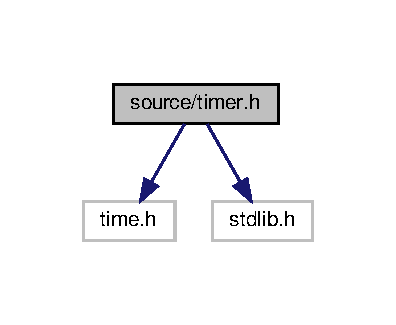
\includegraphics[width=190pt]{timer_8h__incl}
\end{center}
\end{figure}
This graph shows which files directly or indirectly include this file\+:
\nopagebreak
\begin{figure}[H]
\begin{center}
\leavevmode
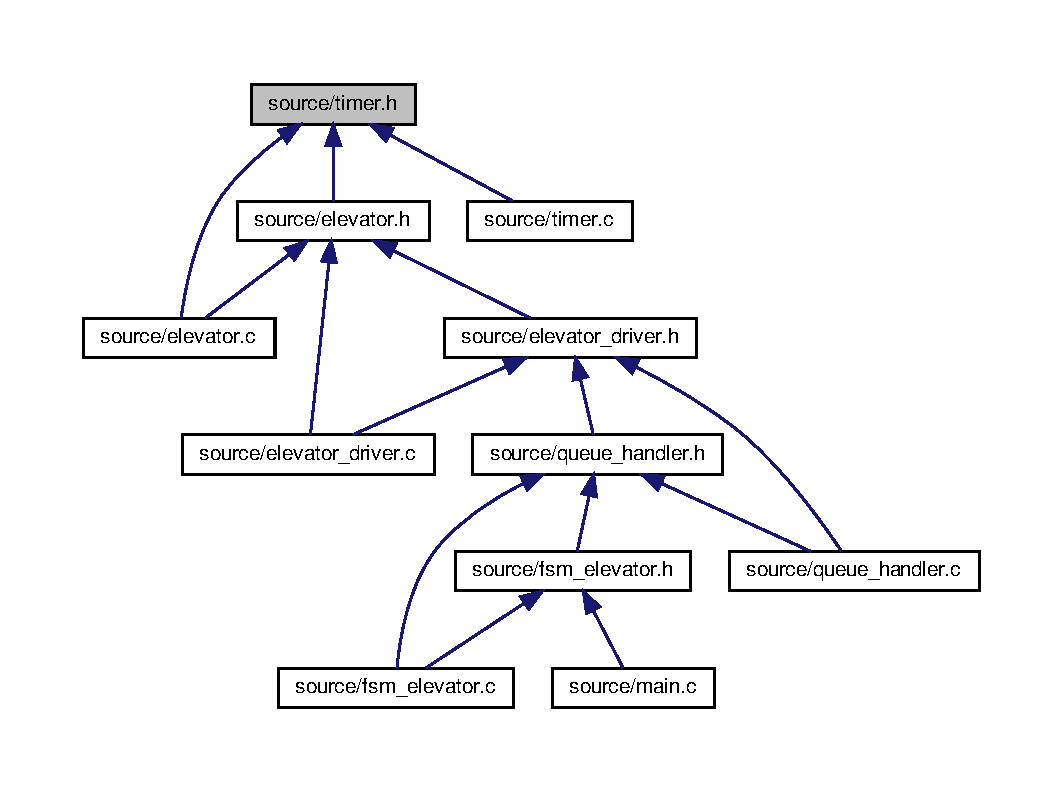
\includegraphics[width=350pt]{timer_8h__dep__incl}
\end{center}
\end{figure}
\subsection*{Macros}
\begin{DoxyCompactItemize}
\item 
\mbox{\Hypertarget{timer_8h_aa8cecfc5c5c054d2875c03e77b7be15d}\label{timer_8h_aa8cecfc5c5c054d2875c03e77b7be15d}} 
\#define {\bfseries T\+R\+UE}~1
\item 
\mbox{\Hypertarget{timer_8h_aa93f0eb578d23995850d61f7d61c55c1}\label{timer_8h_aa93f0eb578d23995850d61f7d61c55c1}} 
\#define {\bfseries F\+A\+L\+SE}~0
\end{DoxyCompactItemize}
\subsection*{Functions}
\begin{DoxyCompactItemize}
\item 
\mbox{\Hypertarget{timer_8h_afaa8b0f43098c4471e98c4733ddb0be3}\label{timer_8h_afaa8b0f43098c4471e98c4733ddb0be3}} 
time\+\_\+t \hyperlink{timer_8h_afaa8b0f43098c4471e98c4733ddb0be3}{timer\+\_\+start\+\_\+time} ()
\begin{DoxyCompactList}\small\item\em Function that returns current time. \end{DoxyCompactList}\item 
int \hyperlink{timer_8h_a0b0053f4a34ba0f1923b6aa691ce338e}{timer\+\_\+three\+\_\+seconds} (time\+\_\+t start\+\_\+time)
\begin{DoxyCompactList}\small\item\em Function that returns 1 if three seconds is passed. \end{DoxyCompactList}\end{DoxyCompactItemize}


\subsection{Detailed Description}
File that contains the timer module. 



\subsection{Function Documentation}
\mbox{\Hypertarget{timer_8h_a0b0053f4a34ba0f1923b6aa691ce338e}\label{timer_8h_a0b0053f4a34ba0f1923b6aa691ce338e}} 
\index{timer.\+h@{timer.\+h}!timer\+\_\+three\+\_\+seconds@{timer\+\_\+three\+\_\+seconds}}
\index{timer\+\_\+three\+\_\+seconds@{timer\+\_\+three\+\_\+seconds}!timer.\+h@{timer.\+h}}
\subsubsection{\texorpdfstring{timer\+\_\+three\+\_\+seconds()}{timer\_three\_seconds()}}
{\footnotesize\ttfamily int timer\+\_\+three\+\_\+seconds (\begin{DoxyParamCaption}\item[{time\+\_\+t}]{start\+\_\+time }\end{DoxyParamCaption})}



Function that returns 1 if three seconds is passed. 

The function takes in a time and returns 1 when the differnce between stat\+\_\+time and current time is bigger or equal to three. 
\begin{DoxyParams}{Parameters}
{\em time} & object start\+\_\+time. \\
\hline
\end{DoxyParams}


Definition at line 12 of file timer.\+c.


%--- End generated contents ---

% Index
\backmatter
\newpage
\phantomsection
\clearemptydoublepage
\addcontentsline{toc}{chapter}{Index}
\printindex

\end{document}
